\documentclass[10pt]{report}

\usepackage{stan-talks}

\begin{document}
\sf%
\vspace*{-12pt}
%
\noindent
\spc{\Huge\bfseries \color{MidnightBlue}{WALNUTS:}}
\\[6pt]
\spc{\LARGE\bfseries \color{MidnightBlue}{Per-leapfrog step size
    adaptation for HMC}}
\\[16pt]
\noindent
\spc{\Large\bfseries \color{MidnightBlue}{Bob Carpenter}}
\\[6pt]
\spc{\large Center for Computational Mathematics}
\\
\spc{\large Flatiron Institute}
\\[12pt]
\vfill
\hfill

\includegraphics[height=0.35in]{img/fi-logo.png}
\qquad

\includegraphics[height=0.5in]{img/stan-logo.png}

\sld{Bayesian statistics with Monte Carlo}
\begin{itemize}
\item Bayesian \myemph{posterior inference} given data $y$ with parameters $\theta$:
\begin{eqnarray*}
  \widehat{\theta} & = & \mathbb{E}[\Theta \mid y]
  \\
  \Pr[E \mid y] & = & \mathbb{E}[\textrm{I}_E(\Theta) \mid y]
  \\
  p(\widetilde{y} \mid y) & = & \mathbb{E}[p(\widetilde{y} \mid
                                \Theta) \mid y]
\end{eqnarray*}
\item Expectations involve \myemph{high-dimensional integrals}.
  $$ \mathbb{E}[f(\Theta) \mid y] = \int_\Theta f(\theta) p(\theta
  \mid y) \textrm{d}\theta. $$
\item (Markov chain) \myemph{Monte Carlo solves integrals} with $\theta^{(m)} \sim p(\theta \mid y).$
  $$ \mathbb{E}[f(\Theta) \mid y] \approx \frac{1}{M} \sum_{m=1}^M
  f(\theta^{(m)}) $$
\end{itemize}

\sld{Why NUTS?}
%
\begin{itemize}
\item Hamiltonian Monte Carlo (HMC, 1985), a Markov chain Monte
  Carlo (MCMC) method, \myemph{scales well in dimension}.
  \begin{subitemize}
  \item integrated autocorrelation time: $\mathcal{O}\left(D^{1/4}\right)$
  \item memory: $\mathcal{O}(D)$)
  \item Hamiltonian \myemph{gradient flow} overcomes diffusive random walk behavior.
  \end{subitemize}
\item Why wasn't HMC in wide use until the \myemph{no-U-turn sampler}
  (NUTS, 2012)?
  \begin{subitemize}
  \item NUTS is fundamental to every probabilistic and differentiable
    programming language: Stan, PyMC, NumPyro, Turing.jl, Blackjax, NIMBLE, ADMB, etc.
  \end{subitemize}
  \vfill
\item A double whammy:
  \begin{subitemize}
  \item HMC is hard to tune; NUTS brought \myemph{self tuning}.
  \item gradients are hard for applications; \myemph{automatic differentiation} makes it easy.
  \end{subitemize}
\end{itemize}

\sld{What is HMC and why is it hard to tune?}
\begin{itemize}
\item Fictitious physical system with \myemph{position} $\theta \in
  \mathbb{R}^D$ and \myemph{momentum} $\rho \in \mathbb{R}^D$:
  \begin{subitemize}
  \item \myemph{Potential} energy: $U(\theta) = - \log p(\theta)$ for
    \myemph{target density} $p(\theta)$
  \item \myemph{Kinetic} energy: $K(\rho) - \log \textrm{normal}(\rho \mid 0, M)$
  \item \myemph{Hamiltonian} (total energy): $H(\theta, \rho) =
    U(\theta) + K(\rho)$, \quad $p(\theta, \rho) = \exp\left( -H(\theta, \rho)\right)$
  \end{subitemize}
\item \myemph{HMC iteration} from position $\theta$:
  \begin{subitemize}
  \item \myemph{Sample momentum}: $\rho \sim \textrm{normal}(0, M)$
  \item \myemph{Evolve Hamiltonian}: from $(\theta, \rho)$ for time $t$
    to $(\theta(t), \rho(t))$ and return $\theta(t)$.
  \end{subitemize}
\item In practice, can't solve exactly, so discretize.
  \begin{subitemize}
  \item \myemph{Simulate:} Take $L$ first-order steps of time $\epsilon = t / L$
    to $(\theta', \rho') \approx (\theta(t), \rho(t))$.
  \item \myemph{Metropolize:} Return $\theta'$ with probability $1 \wedge p(\theta',
      \rho') / p(\theta, \rho)$; \ else return $\theta$.
  \end{subitemize}
\end{itemize}

\sld{Harmonics in HMC}

\begin{minipage}[t]{0.7\textwidth}
  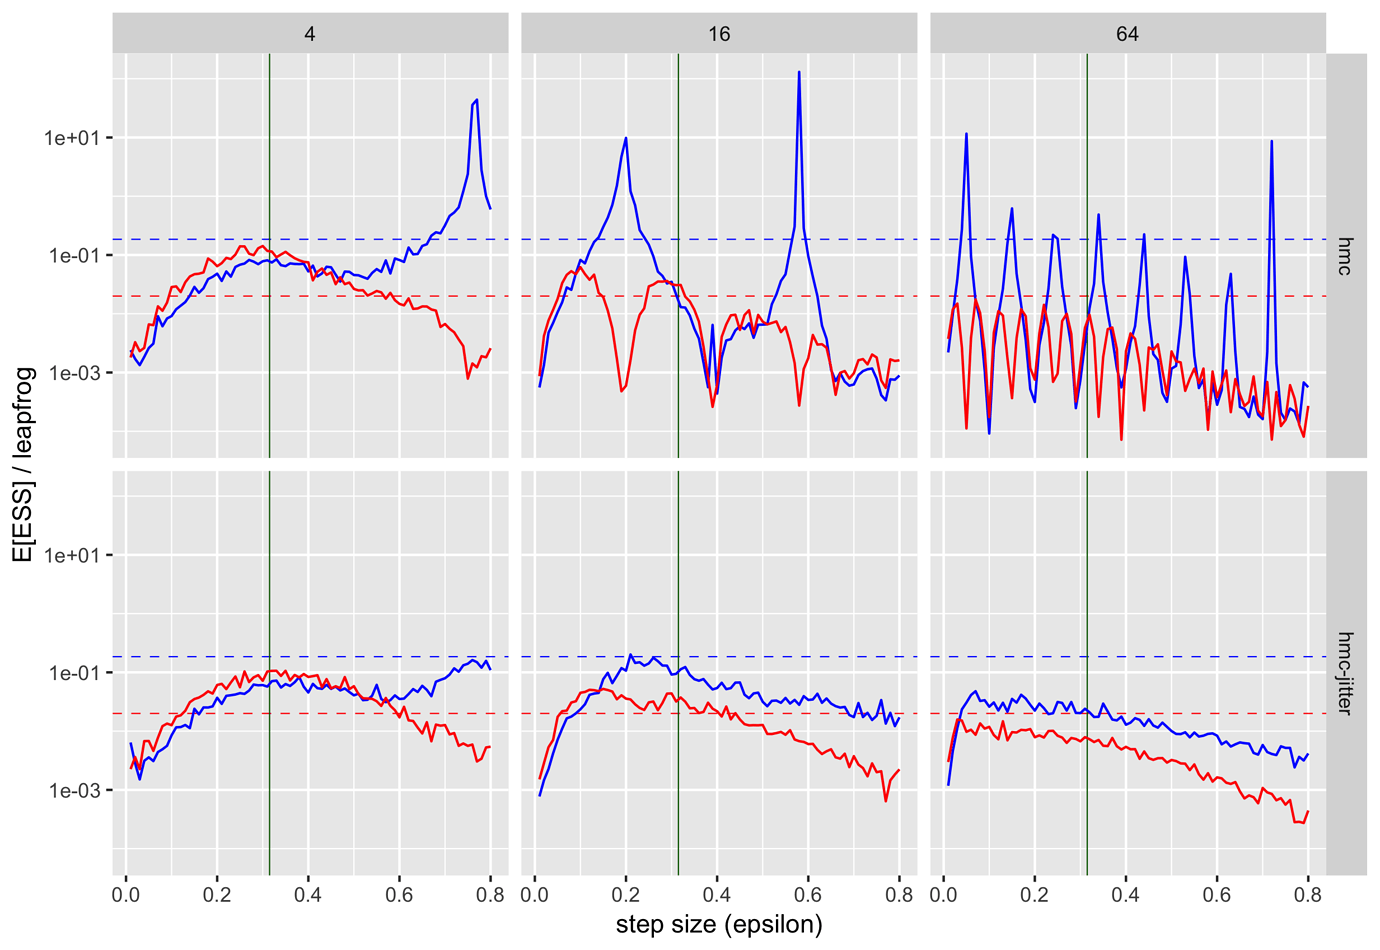
\includegraphics[width=\textwidth]{img/ess-per-leapfrog-jitter-hmc.png}
\end{minipage}%
\begin{minipage}[t]{0.29\textwidth}
  \null\vspace*{-2.5in}
  \begin{subitemize}
  \item \myemph{Target}: 1000-dim standard normal
  \item \myemph{y-axis} (log):  ESS; \\ \myemph{x-axis}: step size
  \item \myemph{red}: $\mathbb{E}[\Theta]$; \\ \myemph{blue}:
    $\mathbb{E}[\Theta^2]$
  \item \myemph{top}: HMC; \\ \myemph{bottom}: jittered time HMC
  \item \myemph{solid}:~HMC,\\ \myemph{dashed}: NUTS
  \end{subitemize}
\end{minipage}

\sld{Multinomial HMC}
\begin{itemize}
\item \myemph{Each iteration} from previous position $\theta(0)$:
  \begin{subitemize}
  \item generate new momentum $\rho(0) \sim \textrm{normal}(0, M)$
  \item generate random steps forward $F \sim \textrm{uniform}(\{ 0, \ldots, L \})$
  \item take $B = L - F$ leapfrog steps backward and $F$ forward from
    $(\theta(0), \rho(0))$
  \item yields $(\theta(n), \rho(n))$ for $-B \leq n \leq F$
    (including initial)
  \item select next state $(\theta(n), \rho(n))$ with probability
    $\null \propto p(\theta(n), \rho(n))$
  \end{subitemize}
\item \myemph{No rejection}, \myemph{no harmonics}, \myemph{no bad
    luck} on Hamiltonian error
  \vfill
\item Straightforward to prove \myemph{detailed balance} (cf. our
  second \textit{GIST} paper)
\end{itemize}

\sld{Naive no-U-turn sampler (NUTS)}
\begin{itemize}
\item Go forward and backward and time at random
\item doubling number of steps each time
\item until a U-turn between ends or a sub-U-turn within doubled steps
\item select next state proportional to density (a la multinomial HMC)
  \vfill
\item Original NUTS: slice sample rather than multinomial sample
\end{itemize}

\sld{Biased-progressive NUTS}
\begin{itemize}
\item Keep a selected state, initially $(\theta(0), \rho(0))$
\item At each doubling from $M$ to $2M$ states:
  \begin{subitemize}
    \item Metropolis probability of updating state:
      $$1 \wedge \dfrac{\sum_{m=M+1}^{2M} p(\theta(m), \rho(m))}
                       {\sum_{m=1}^M p(\theta(m), \rho(m))}$$
      \item If upding, select new state $(\theta(m), \rho(m))$
        porportional to density $\propto p(\theta(m), \rho(m))$
        for $M < m \leq 2M$.
  \end{subitemize}
\item Return final selected item.
\end{itemize}

\sld{QR code for GitHub: C++ \& paper link}
\spc
\noindent
\begin{minipage}[t]{0.35\textwidth}

\includegraphics[width=\textwidth]{img/qr-code.pdf}
\end{minipage}
\quad
\begin{minipage}[t]{0.6\textwidth}
  \vspace*{-1.55in}
  {\small Nawawf Bou-Rabee, Bob Carpenter, Tore S. Kleppe, and Sifan Liu.
      2025. \myemph{WALNUTS: The Within-Orbit Adaptive Leapfrog No-U-Turn
      Sampler}. \textit{arXiv} 2506.18746.}
      \\[12pt]
      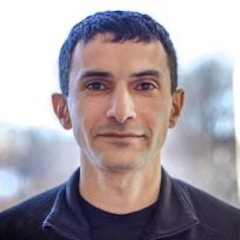
\includegraphics[width=0.25\textwidth]{img/nawaf.jpg}
      \hfill
      
\includegraphics[width=0.25\textwidth]{img/tore.png}
      \hfill
      
\includegraphics[width=0.25\textwidth]{img/sifan.jpg}
\end{minipage}
\hfill
\null



\end{document}